\documentclass[aspectratio=169,11pt]{beamer}

% ============================================================
% PACKAGES
% ============================================================

\usepackage[T1]{fontenc}
\usepackage{lmodern}
\usepackage{amsmath,amssymb}
\usepackage{booktabs}
\usepackage{graphicx}
\usepackage{tikz}
\usepackage{hyperref}

\usetikzlibrary{
	positioning,
	shapes.geometric,
	shadows,
	calc,
	arrows.meta
}

% ============================================================
% BEAMER SETTINGS
% ============================================================

\setbeamertemplate{navigation symbols}{}

\setbeamertemplate{blocks}[rounded][shadow=true]

% ============================================================
% COLORS
% ============================================================

\definecolor{CyberDark}{RGB}{8,12,20}
\definecolor{CyberBlue}{RGB}{20,110,190}
\definecolor{CyberCyan}{RGB}{40,210,220}
\definecolor{CyberWhite}{RGB}{235,240,245}
\definecolor{CyberGray}{RGB}{150,160,175}
\definecolor{CyberRed}{RGB}{220,70,80}

% ============================================================
% GLOBAL COLORS
% ============================================================

\setbeamercolor{normal text}{
	fg=CyberWhite,
	bg=CyberDark
}

\setbeamercolor{frametitle}{
	fg=CyberCyan,
	bg=CyberDark
}

\setbeamercolor{title}{
	fg=CyberCyan
}

\setbeamercolor{subtitle}{
	fg=CyberGray
}

\setbeamercolor{author}{
	fg=CyberWhite
}

\setbeamercolor{institute}{
	fg=CyberGray
}

\setbeamercolor{date}{
	fg=CyberGray
}

\setbeamercolor{block title}{
	fg=CyberWhite,
	bg=CyberBlue
}

\setbeamercolor{block body}{
	fg=CyberWhite,
	bg=CyberDark
}

% ============================================================
% BACKGROUND
% ============================================================

\setbeamertemplate{background}
{
	\begin{tikzpicture}[remember picture,overlay]
		
		% Main background
		\fill[CyberDark]
		(current page.south west)
		rectangle
		(current page.north east);
		
		% Perspective grid
		\foreach \x in {-8,-7.5,...,8}
		{
			\draw[CyberBlue,opacity=0.08]
			([xshift=\x cm]current page.south)
			--
			([xshift=\x cm,yshift=2cm]current page.center);
		}
		
		\foreach \y in {0,0.5,...,5}
		{
			\draw[CyberBlue,opacity=0.06]
			(current page.south west |- current page.south)
			--
			(current page.south east |- current page.south);
		}
		
		% Decorative nodes
		
		\fill[CyberCyan,opacity=.35]
		([xshift=-1cm,yshift=1cm]current page.north east)
		circle (0.08cm);
		
		\fill[CyberCyan,opacity=.25]
		([xshift=-3cm,yshift=2cm]current page.north east)
		circle (0.05cm);
		
		\fill[CyberBlue,opacity=.35]
		([xshift=1cm,yshift=2cm]current page.south west)
		circle (0.08cm);
		
	\end{tikzpicture}
}

% ============================================================
% FRAME TITLE
% ============================================================

\setbeamertemplate{frametitle}
{
	\vspace{0.35cm}
	
	
\begin{tikzpicture}
		\node[
		anchor=west,
		font=\Large\bfseries,
		text=CyberCyan
		]
		{\insertframetitle};
		
		\draw[
		CyberBlue,
		line width=1pt
		]
		(0,-0.18) -- (10,-0.18);
	\end{tikzpicture}
	
	\vspace{0.15cm}
}

% ============================================================
% FOOTER
% ============================================================

\setbeamertemplate{footline}
{
	\begin{tikzpicture}[remember picture,overlay]
		
		\draw[
		CyberBlue,
		opacity=.5,
		line width=.5pt
		]
		([yshift=0.35cm]current page.south west)
		--
		([yshift=0.35cm]current page.south east);
		
		\node[
		anchor=south west,
		text=CyberGray,
		font=\tiny
		]
		at ([xshift=.35cm,yshift=.05cm]current page.south west)
		{Peter M. Ngugi | PhD Computer Science};
		
		\node[
		anchor=south east,
		text=CyberCyan,
		font=\tiny
		]
		at ([xshift=-.35cm,yshift=.05cm]current page.south east)
		{\insertframenumber{} / \inserttotalframenumber};
		
	\end{tikzpicture}
}

% ============================================================
% TITLE PAGE
% ============================================================

\setbeamertemplate{title page}
{
	
	\begin{tikzpicture}[remember picture,overlay]
		
		% 3D cube
		
		\draw[
		CyberCyan,
		line width=1.5pt,
		opacity=.9
		]
		([xshift=5.5cm,yshift=1cm]current page.center)
		--
		([xshift=8cm,yshift=2.5cm]current page.center)
		--
		([xshift=8cm,yshift=5cm]current page.center)
		--
		([xshift=5.5cm,yshift=3.5cm]current page.center)
		-- cycle;
		
		\draw[
		CyberBlue,
		line width=1.5pt,
		opacity=.8
		]
		([xshift=5.5cm,yshift=1cm]current page.center)
		--
		([xshift=5.5cm,yshift=3.5cm]current page.center);
		
		\draw[
		CyberBlue,
		line width=1.5pt,
		opacity=.8
		]
		([xshift=8cm,yshift=2.5cm]current page.center)
		--
		([xshift=8cm,yshift=5cm]current page.center);
		
		\draw[
		CyberBlue,
		line width=1.5pt,
		opacity=.8
		]
		([xshift=5.5cm,yshift=3.5cm]current page.center)
		--
		([xshift=8cm,yshift=5cm]current page.center);
		
		% Network nodes
		
		\foreach \x/\y in
		{
			4.8/0.7,
			6.5/1.8,
			8.5/3,
			6/4,
			9/4.7
		}
		{
			\fill[CyberCyan]
			([xshift=\x cm,yshift=\y cm]current page.south west)
			circle (0.07cm);
		}
		
	\end{tikzpicture}
	
	\vspace*{0.7cm}
	
	{\usebeamerfont{title}
		\color{CyberCyan}
		\inserttitle
	}
	
	\vspace{0.35cm}
	
	{\usebeamerfont{subtitle}
		\color{CyberGray}
		\insertsubtitle
	}
	
	\vspace{1cm}
	
	{\large
		\color{CyberWhite}
		\insertauthor
	}
	
	\vspace{0.25cm}
	
	{\small
		\color{CyberGray}
		\insertinstitute
	}
	
	\vspace{0.25cm}
	
	{\small
		\color{CyberGray}
		\insertdate
	}
	
}

% ============================================================
% PRESENTATION INFORMATION
% ============================================================

\title[
AI Cybercrime Forensics
]
{
	Forensics for Cybercrimes Committed Using Artificial Intelligence
}

\subtitle{
	A Digital Forensic Framework for AI-Assisted Cybercrime
}

\author{
	Peter M. Ngugi
}

\institute{
	PhD in Computer Science\\
	Zetech University
}

\date{
	2026
}

% ============================================================
% DOCUMENT
% ============================================================

\begin{document}
	
	% ------------------------------------------------------------
	% TITLE
	% ------------------------------------------------------------
	
	\begin{frame}[plain]
		
		\titlepage
		
	\end{frame}
	
	% ------------------------------------------------------------
	% CONTENT
	% ------------------------------------------------------------
	
	\begin{frame}{Research Context}
		
		Artificial Intelligence is changing the cybercrime landscape.
		
		\vspace{0.4cm}
		
		\begin{columns}
			
			\column{0.48\textwidth}
			
			\begin{block}{Traditional Cybercrime}
				\begin{itemize}
					\item Human-controlled systems
					\item Identifiable devices
					\item Conventional malware
					\item Established forensic procedures
				\end{itemize}
			\end{block}
			
			\column{0.48\textwidth}
			
			\begin{block}{AI-Assisted Cybercrime}
				\begin{itemize}
					\item Automated attacks
					\item Synthetic identities
					\item AI-generated content
					\item Autonomous decision-making
				\end{itemize}
			\end{block}
			
		\end{columns}
		
	\end{frame}
	
	% ------------------------------------------------------------
	
	\begin{frame}{The Forensic Challenge}
		
		\begin{center}
			
			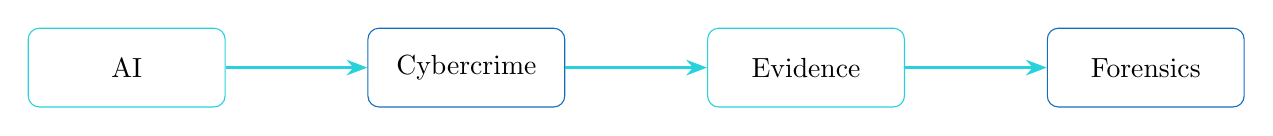
\begin{tikzpicture}[node distance=1.8cm]
				
				\node[
				draw=CyberCyan,
				rounded corners,
				minimum width=2.5cm,
				minimum height=1cm
				]
				(AI)
				{AI};
				
				\node[
				draw=CyberBlue,
				rounded corners,
				minimum width=2.5cm,
				minimum height=1cm,
				right=of AI
				]
				(CYBER)
				{Cybercrime};
				
				\node[
				draw=CyberCyan,
				rounded corners,
				minimum width=2.5cm,
				minimum height=1cm,
				right=of CYBER
				]
				(EVID)
				{Evidence};
				
				\node[
				draw=CyberBlue,
				rounded corners,
				minimum width=2.5cm,
				minimum height=1cm,
				right=of EVID
				]
				(FORENS)
				{Forensics};
				
				\draw[
				->,
				>=Stealth,
				CyberCyan,
				line width=1pt
				]
				(AI) -- (CYBER);
				
				\draw[
				->,
				>=Stealth,
				CyberCyan,
				line width=1pt
				]
				(CYBER) -- (EVID);
				
				\draw[
				->,
				>=Stealth,
				CyberCyan,
				line width=1pt
				]
				(EVID) -- (FORENS);
				
			\end{tikzpicture}
			
		\end{center}
		
		\vspace{0.7cm}
		
		The central question is not merely:
		
		\begin{center}
			\Large
			\textit{What happened?}
		\end{center}
		
		but also:
		
		\begin{center}
			\Large
			\textit{Who or what caused it, and can we prove it?}
		\end{center}
		
	\end{frame}
	
	% ------------------------------------------------------------
	
	\begin{frame}{Forensic Evidence Pipeline}
		
		\begin{center}
			
			
\begin{tikzpicture}[node distance=1.1cm]
				
				\node[
				draw=CyberCyan,
				rounded corners,
				minimum width=2.1cm,
				minimum height=.8cm
				]
				(C)
				{Collection};
				
				\node[
				draw=CyberBlue,
				rounded corners,
				minimum width=2.1cm,
				minimum height=.8cm,
				right=of C
				]
				(P)
				{Preservation};
				
				\node[
				draw=CyberCyan,
				rounded corners,
				minimum width=2.1cm,
				minimum height=.8cm,
				right=of P
				]
				(A)
				{Authentication};
				
				\node[
				draw=CyberBlue,
				rounded corners,
				minimum width=2.1cm,
				minimum height=.8cm,
				right=of A
				]
				(AN)
				{Analysis};
				
				\node[
				draw=CyberCyan,
				rounded corners,
				minimum width=2.1cm,
				minimum height=.8cm,
				right=of AN
				]
				(AT)
				{Attribution};
				
				\draw[
				->,
				CyberCyan,
				line width=1pt
				]
				(C) -- (P);
				
				\draw[
				->,
				CyberCyan,
				line width=1pt
				]
				(P) -- (A);
				
				\draw[
				->,
				CyberCyan,
				line width=1pt
				]
				(A) -- (AN);
				
				\draw[
				->,
				CyberCyan,
				line width=1pt
				]
				(AN) -- (AT);
				
			\end{tikzpicture}
			
		\end{center}
		
	\end{frame}
	
	% ------------------------------------------------------------
	
	\begin{frame}{Formalising the Evidence Problem}
		
		Let
		
		\[
		E = \{e_1,e_2,\ldots,e_n\}
		\]
		
		represent the set of collected digital evidence.
		
		Let
		
		\[
		A \subseteq E
		\]
		
		represent evidence that has successfully passed
		an authentication process.
		
		Therefore,
		
		\[
		A \subseteq E
		\]
		
		and
		
		\[
		e_i \in A
		\Rightarrow
		e_i \text{ satisfies the defined authentication criteria.}
		\]
		
		\vspace{0.5cm}
		
		This provides a formal basis for reasoning about
		digital evidence rather than relying solely on
		descriptive analysis.
		
	\end{frame}
	
	% ------------------------------------------------------------
	
	\begin{frame}{Research Objectives}
		
		\begin{enumerate}
			
			\item Examine how AI can facilitate cybercrime.
			
			\vspace{0.2cm}
			
			\item Identify limitations in existing digital forensic
			approaches.
			
			\vspace{0.2cm}
			
			\item Investigate evidence provenance and integrity.
			
			\vspace{0.2cm}
			
			\item Develop a forensic framework for AI-assisted
			cybercrime.
			
			\vspace{0.2cm}
			
			\item Evaluate the proposed framework.
			
		\end{enumerate}
		
	\end{frame}
	
	% ------------------------------------------------------------
	
	\begin{frame}{Expected Contribution}
		
		\begin{center}
			
			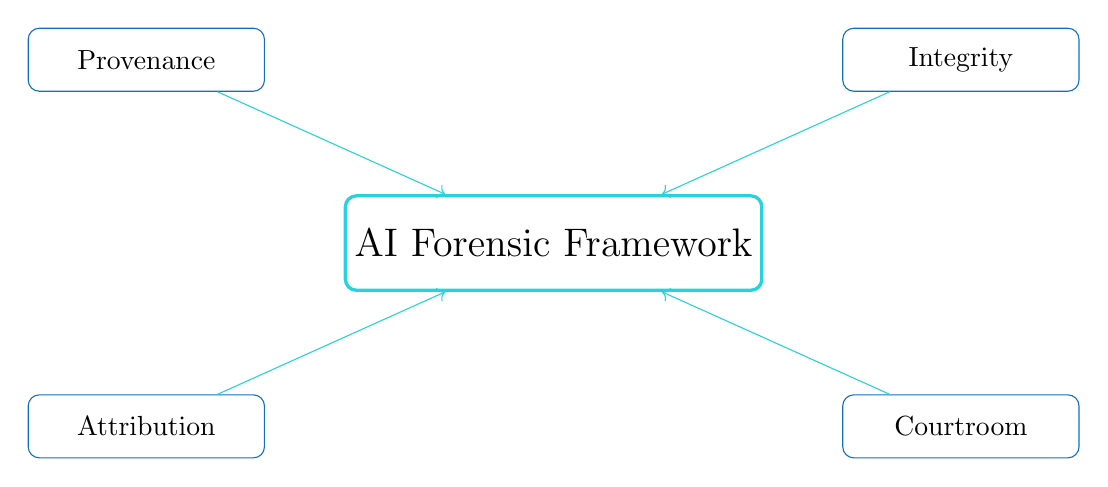
\begin{tikzpicture}
				
				\node[
				draw=CyberCyan,
				line width=1.2pt,
				rounded corners,
				minimum width=4cm,
				minimum height=1.2cm
				]
				(F)
				{\Large AI Forensic Framework};
				
				\node[
				draw=CyberBlue,
				rounded corners,
				minimum width=3cm,
				minimum height=.8cm,
				above left=1.3cm and 1cm of F
				]
				(P)
				{Provenance};
				
				\node[
				draw=CyberBlue,
				rounded corners,
				minimum width=3cm,
				minimum height=.8cm,
				above right=1.3cm and 1cm of F
				]
				(I)
				{Integrity};
				
				\node[
				draw=CyberBlue,
				rounded corners,
				minimum width=3cm,
				minimum height=.8cm,
				below left=1.3cm and 1cm of F
				]
				(A)
				{Attribution};
				
				\node[
				draw=CyberBlue,
				rounded corners,
				minimum width=3cm,
				minimum height=.8cm,
				below right=1.3cm and 1cm of F
				]
				(C)
				{Courtroom};
				
				\draw[CyberCyan,->] (P) -- (F);
				\draw[CyberCyan,->] (I) -- (F);
				\draw[CyberCyan,->] (A) -- (F);
				\draw[CyberCyan,->] (C) -- (F);
				
			\end{tikzpicture}
			
		\end{center}
		
	\end{frame}
	
	% ------------------------------------------------------------
	
	\begin{frame}{Conclusion}
		
		\begin{block}{Central Argument}
			
			AI changes not only how cybercrimes can be committed,
			but also how digital evidence must be interpreted,
			authenticated and attributed.
			
		\end{block}
		
		\vspace{0.7cm}
		
		\begin{center}
			
			\[
			\boxed{
				AI
				+
				Cybercrime
				+
				Digital\ Forensics
				+
				Evidence
			}
			\]
			
		\end{center}
		
	\end{frame}
	
	% ------------------------------------------------------------
	
	\begin{frame}[plain]
		
		\begin{center}
			
			\vspace{1.5cm}
			
			{\Huge
				\color{CyberCyan}
				\textbf{Thank You}
			}
			
			\vspace{0.8cm}
			
			{\Large
				\color{CyberWhite}
				Questions \& Discussion
			}
			
			\vspace{1.2cm}
			
			{\small
				Peter M. Ngugi\\
				PhD in Computer Science\\
				Zetech University
			}
			
		\end{center}
		
	\end{frame}
	
\end{document}